% The model in the style of Figure 3 of van Knippenberg et al. (2021): plain
% black boxes, the agent's layer stack zoomed from Agent 1, and the loop through
% the environment. Added to theirs: the move score and value head on top of the
% message passing, and conflict resolution between the agents and the
% environment. The worded version is architecture.tex, the full network
% architecture_detail.tex.
% Build:  latexmk -pdf architecture_compact.tex, then copy the pdf to Images/.
\documentclass[border=2pt]{standalone}
\usepackage{lmodern}
\usepackage[T1]{fontenc}
\usepackage{amsmath,amssymb}
\usepackage{tikz}
\usetikzlibrary{positioning,fit,arrows.meta,calc}

\tikzset{
  box/.style={draw, line width=0.6pt, align=center, inner sep=3pt,
              minimum height=0.6cm, font=\small},
  flow/.style={-{Latex[length=2mm]}, line width=0.6pt},
  lbl/.style={font=\footnotesize},
}

\begin{document}
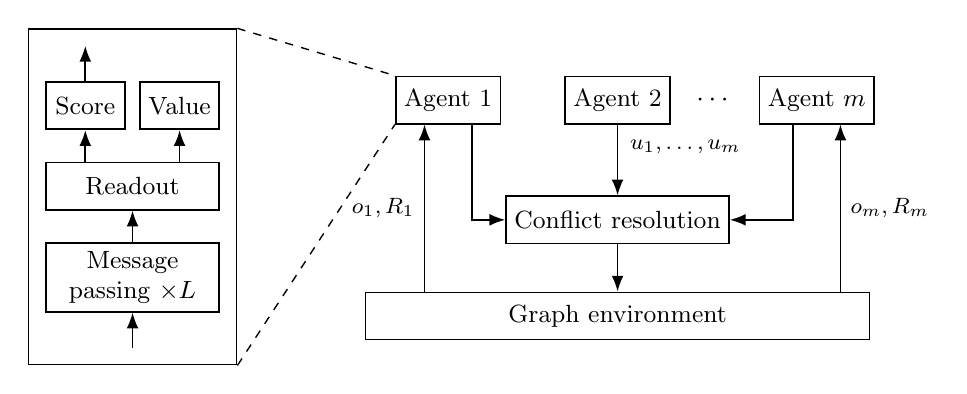
\begin{tikzpicture}
  % ---------------------------------------------------------- the agent model
  \node[box, minimum width=2.2cm] (mp) {Message\\ passing $\times L$};
  \node[box, minimum width=2.2cm, above=0.4cm of mp] (ro) {Readout};
  \node[box, minimum width=1.0cm, above=0.4cm of ro.north west, anchor=south west] (sc) {Score};
  \node[box, minimum width=1.0cm, above=0.4cm of ro.north east, anchor=south east] (vf) {Value};
  \coordinate (inlet) at ($(mp.south)+(0,-0.45)$);
  \draw[flow] (inlet) -- (mp);
  \draw[flow] (mp) -- (ro);
  \draw[flow] (ro.north -| sc) -- (sc);
  \draw[flow] (ro.north -| vf) -- (vf);
  \coordinate (outlet) at ($(sc.north)+(0,0.45)$);
  \draw[flow] (sc) -- (outlet);
  \node[draw, line width=0.6pt, inner sep=6pt,
        fit=(mp)(sc)(vf)(inlet)(outlet)] (model) {};

  % ---------------------------------------------------------- agents and loop
  \node[box, right=2.0cm of model.north east, anchor=north west, yshift=-0.6cm] (a1) {Agent 1};
  \node[box, right=0.8cm of a1] (a2) {Agent 2};
  \node[right=0.2cm of a2] (dots) {$\cdots$};
  \node[box, right=0.2cm of dots] (am) {Agent $m$};
  \node[box, below=0.9cm of a2.south, anchor=north] (cr) {Conflict resolution};
  \node[box, below=0.6cm of cr, minimum width=6.4cm] (env) {Graph environment};

  % observation and reward up to each agent, along the outer sides
  \draw[flow] (env.north -| a1) ++(-0.3,0) -- ($(a1.south)+(-0.3,0)$)
    node[pos=0.5, left, lbl] {$o_1, R_1$};
  \draw[flow] (env.north -| am) ++(0.3,0) -- ($(am.south)+(0.3,0)$)
    node[pos=0.5, right, lbl] {$o_m, R_m$};
  % each agent's move down into conflict resolution, then into the environment
  \draw[flow] ($(a1.south)+(0.3,0)$) |- (cr.west);
  \draw[flow] (a2.south) -- (a2.south |- cr.north);
  \draw[flow] ($(am.south)+(-0.3,0)$) |- (cr.east);
  \draw[flow] (cr) -- (env);
  \node[lbl, right=1pt of a2.south, anchor=north west, yshift=-2pt] {$u_1, \dots, u_m$};

  % zoom lines from Agent 1 to the model
  \draw[dashed, line width=0.5pt] (model.north east) -- (a1.north west);
  \draw[dashed, line width=0.5pt] (model.south east) -- (a1.south west);
\end{tikzpicture}
\end{document}
